\documentclass{article}
\usepackage{amsmath, amssymb, tikz, tkz-euclide, tcolorbox, array, sfmath, enumerate, pgfplots, multicol}
\renewcommand{\familydefault}{\sfdefault}
\pgfplotsset{compat=newest}
\usetikzlibrary{arrows.meta}
\everymath{\displaystyle}
\tikzset{>=stealth}
\newcounter{example}[section]
\newenvironment{example}[1][]{\refstepcounter{example}\par\medskip
   {\color{red}\textbf{Example~\theexample. #1}}}{\medskip}
\usepackage[top = 0.25in, bottom = 0.25in, left = 1in, right = 1in]{geometry}
\pagestyle{empty}
\raggedright

\begin{document}

\section*{Absolute Value Inequalities}

\begin{tcolorbox}[colframe=orange!70!white, coltitle=black, title=\textbf{Summary}]
\begin{enumerate}
    \item Absolute value inequalities are examples of compound inequalities.
    \item Check the answers you get in the original problem.
\end{enumerate}
\end{tcolorbox}
\bigskip 

Absolute value inequalities are similar to absolute value equations.	


\subsection*{Less Than (\boldmath{$<$}) and Less Than or Equal To (\boldmath{$\leq$})}

For $|x| < 2$, we want all values of $x$ that are \textbf{less than 2 units from 0} on a number line:	\newline\\	

\begin{center}
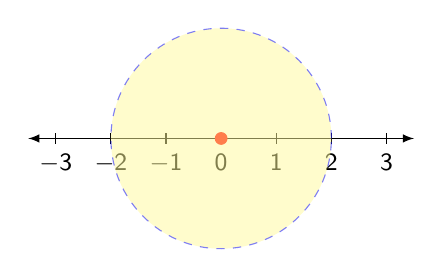
\begin{tikzpicture}[scale=0.7]
 	\draw [<->, > = latex] (-3.5,0) -- (3.5,0);
	\foreach \x in {-3,-2,...,3}
	\draw (\x, -0.1) -- (\x, 0.1);
	\foreach \x in {-3,-2,...,3}
	\node at (\x, -0.1) [below] {\small $\x$};
	\draw [red, fill=red] (0,0) circle [radius = 3pt];
	\draw [blue, dashed, fill=yellow!40, opacity=0.5] (0,0) circle [radius = 2cm];
\end{tikzpicture}
\end{center}
\bigskip 

\begin{center}
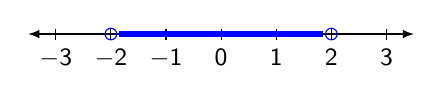
\begin{tikzpicture}[scale=0.7]
 	\draw [<->, > = latex] (-3.5,0) -- (3.5,0);
	\foreach \x in {-3,-2,...,3}
	\draw (\x, -0.1) -- (\x, 0.1);
	\foreach \x in {-3,-2,...,3}
	\node at (\x, -0.1) [below] {\small $\x$};
	\draw (-2,0) [color = blue!120] circle (3pt);
	\draw (2,0) [color = blue!120] circle (3pt);
	\draw [line width = 2, color = blue!120, shorten <= 3pt, shorten >= 3pt] (-2,0) -- (2,0);
\end{tikzpicture}
\end{center}

\[|x| < 2 \text{ means } -2 < x < 2\]
\vspace{-10pt}
\begin{center}
    or
\end{center}

\[x > -2 \quad \text{AND} \quad x < 2 \]
\bigskip 

\begin{example}
Solve and graph each.
\begin{enumerate}[(a)]
\begin{multicols}{3}
    \item $|2x-2| < 5$      
    \item $|x-9| \leq 2.9$  
    \item $|x+2| \leq -1$  
\end{multicols}
\end{enumerate}
\end{example}

\newpage 

\subsection*{Greater Than (\boldmath{$>$}) and Greater Than or Equal To (\boldmath{$\geq$})}

For $|x| > 2$, we want all the values of $x$ that are \textbf{greater than 2 units from 0} on a number line.	\newline\\	

\begin{center}
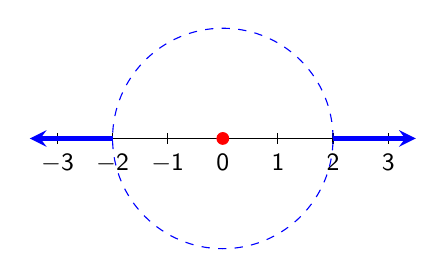
\begin{tikzpicture}[scale=0.7]
 	\draw [<->, > = latex] (-3.5,0) -- (3.5,0);
	\foreach \x in {-3,-2,...,3}
	\draw (\x, -0.1) -- (\x, 0.1);
	\foreach \x in {-3,-2,...,3}
	\node at (\x, -0.1) [below] {\small $\x$};
	\draw [red, fill=red] (0,0) circle [radius = 3pt];
	\draw [blue, dashed] (0,0) circle [radius = 2cm];
	\draw [->, ultra thick, blue] (-2,0) -- (-3.5,0);
	\draw [->, ultra thick, blue] (2,0) -- (3.5,0);
\end{tikzpicture}
\end{center}
\bigskip 

\begin{center}
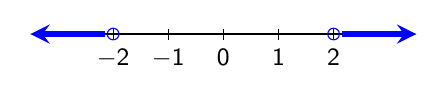
\begin{tikzpicture}[scale=0.7]
	\draw [<->, > = latex] (-3.5,0) -- (3.5,0);
	\foreach \x in {-2,-1,0,1,2}
	\draw (\x, -0.1) -- (\x, 0.1);
	\foreach \x in {-2,-1,0,1,2}
	\node at (\x, -0.1) [below] {\small $\x$};
	\draw (-2,0) [color = blue!120] circle (3pt);
	\draw (2,0) [color = blue!120] circle (3pt);
	\draw [->, line width = 2, color = blue!120, shorten <= 3pt] (-2,0) -- (-3.5,0);
	\draw [->, line width = 2, color = blue!120, shorten <= 3pt] (2,0) -- (3.5,0);	
\end{tikzpicture}
\end{center}

\[|x| > 2 \text{ means that } x < -2 \text{ or } x > 2 \]
\bigskip 

\begin{example}
Solve and graph each.
\begin{enumerate}[(a)]
\begin{multicols}{3}
    \item $|2x+3| \geq 5$  
    \item $|-2x-5| > 3$     
    \item $|2x+2| > -2$  
\end{multicols}
\end{enumerate}
\end{example}

\end{document}
